\section{Theorie}
\label{sec:Theorie}

\subsection{Energieniveaus der Rubidiumisotope}
Rubidium ist ein Alkalimetall und besitzt somit ein Elektron in der Valenzschale.
Näherungsweise wird Rubidium durch das Wasserstoff-Atommodell beschrieben.
In diesem Experiment wird ein Gasgemisch aus den Rubidiumisotopen $^{87}\text{Rb}$ und $^{85}\text{Rb}$ betrachtet.
Der Spin des Elektrons beträgt $S=1/2$.
Anders als bei dem Elektronspin unterscheidet sich der Kern signifikant von einem Wasserstoffatom und führt zu einer veränderten Aufspaltung der Energieniveaus.
Die Isotope weisen aufgrund der unterschiedlichen Nukleonenanzahl einen unterschiedlichen Kernspin $I$ auf, wobei $I=3/2$ für $^{87}\text{Rb}$ und $I=5/2$ für $^{85}\text{Rb}$ gilt.
\\
Die Aufspaltung der Energieniveaus beider Isotope ist in \autoref{fig:energieniveaus} dargestellt.
\begin{figure}
    \centering
    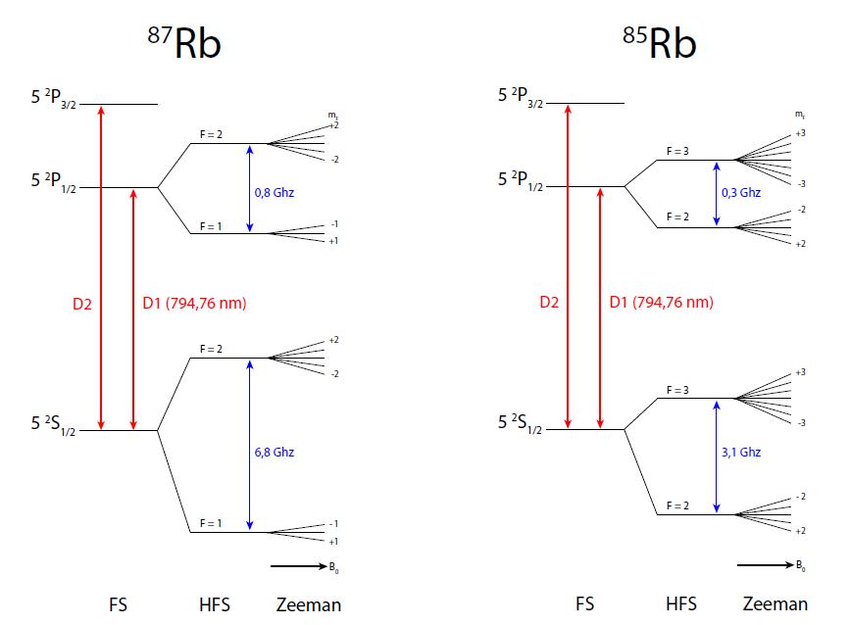
\includegraphics[width=1\textwidth]{content/img/energieniveaus2.png}
    \caption{Schematische Darstellung der Energieniveaus des $^{87}\text{Rb}$- und $^{85}\text{Rb}$-Isotops, 
    wobei die Feinstruktur(\textbf{FS}), die Hyperfeinstruktur(\textbf{HFS}) und die Aufspaltung durch den \textbf{Zeeman}-Effekt betrachtet werden. \cite{borgo}}
    \label{fig:energieniveaus}
\end{figure}
Im folgenden wird die Feinstruktur(\textbf{FS}), die Hyperfeinstruktur(\textbf{HFS}) und die Aufspaltung durch den \textbf{Zeeman}-Effekt der Energieniveaus behandelt.
\\
Die Kreisbewegung des Elektrons um den Atomkern erzeugt ein magnetisches Moment, das mit dem Spin wechselwirkt.
Diese Wechselwirkung wird als Spin-Bahn-Kopplung bezeichnet und resultiert in einer feineren Aufspaltung, der sog. \textbf{Feinstruktur}.
\\
Ein Zustand kann mithilfe der spektroskopischen Notation $^\text{2S+1}\text{L}_\text{J}$ angegeben werden.
Hierbei beschreibt $S$ den Spin, $L$ (=S,P,D,F,...) den Bahndrehimpuls und $\vec{J} = \vec{L} + \vec{S}$ den Gesamtdrehimpuls.
Die Quantenzahl $J$ kann Werte von $|L-S|$ bis $|L+S|$ annehmen.
\\
Das magnetische Moment des Elektrons wechselwirkt ebenfalls mit dem Kernspin $I$.
Dies führt zu einer weiteren Aufspaltung, der \textbf{Hyperfeinstruktur}.
Eine weitere Quantenzahl, der Gesamtdrehimpuls $\vec{F} = \vec{I} + \vec{J}$ wird zur Beschreibung der Hyperfeinstruktur verwendet.
$F$ nimmt dabei ganzzahlige Werte von $|J-I|$ bis $|J+I|$ an.
Die Zustände auf dem gleichen $F$-Niveau weisen nur geringe Energieunterschiede auf.
\\
Wird nun ein externes Magnetfeld angelegt, so erfahren die magnetischen Dipole eine Kraft die abhängig von der Ausrichtung des Dipols ist.
Das Phänomen wird als \textbf{Zeeman-Effekt} bezeichnet und resultiert in der gezeigten Aufspaltung, welche über die magnetische Quantenzahl $m \in {-F, F}$ beschrieben wird.
Für ein hinreichend schwaches Magnetfeld wird die Zeeman-Aufspaltung durch
\begin{equation}
    E_Z = g_F \mu_B B m
\end{equation}
beschrieben.
Die Energie hängt dabei von dem Betrag des angelegten Magnetfeldes $B$, dem Landé-Faktor $g_F$ und der magnetischen Quantenzahl $m$ ab.
Das Bohrsche Magneton
\begin{equation}
    \mu_B = \frac{e \hbar}{2 m_e}
\end{equation}
ist dabei eine über die Naturkonstanten Elektronenladung $e$, Elektronenmasse $m_e$ und das reduzierte plancksche Wirkungsquantum $\hbar$ definierte Größe.
Die Energiedifferenzen zwischen zwei Zeemanaufspaltungen ergibt sich als Landé-Faktor $g_F$
\begin{align}
    g_F &= g_J \frac{F(F+1) + J(J+1) - I(I+1)}{2F(F+1)} \label{eqn:g_F} \\
    \text{mit} \quad g_J &= 1 + \frac{J(J+1) + S(S+1) - L(L+1)}{2J(J+1)} \label{eqn:g_J}
\end{align}
und ist somit allein durch die Quantenzahlen gegeben.


\FloatBarrier
\subsection{Der quadratische Zeeman-Effekt}
\subsection{Das optische Pumpen}